\chapter{Introduction to Optimization and Evolutionary Computation}

  Genetic algorithms (GAs) are population-based search methods inspired by natural selection and genetics. They maintain a population of candidate solutions encoded as strings, iteratively producing new generations by selecting the fittest individuals, recombining their information, and occasionally introducing random variation. Although stochastic in their operators, GAs are not blind random walks: they retain and exploit historical information about good solutions to generate promising new search points and thereby drive efficient exploration and exploitation of complex spaces.

  This family of methods was developed from foundational work by Holland and colleagues to both model adaptive processes observed in nature and to design artificial systems that embody those mechanisms. A central aim has been robustness—the ability to balance efficiency with reliability across a wide range of problem environments—which makes GAs attractive when redesign costs are high or when problem structure violates common assumptions (e.g., continuity, differentiability, or unimodality). Because they are conceptually simple, widely applicable, and empirically effective in optimization and control, genetic algorithms have become a practical tool across engineering, science, and business domains \cite{goldberg1989genetic}.

  To place genetic algorithms in context, we first give a concise definition of optimization — the class of problems GAs are commonly used to solve.
    We define optimization as the process of finding the best solution from a set of available alternatives. In mathematical terms, an optimization problem can be formulated as:

  \begin{equation}
  \begin{aligned}
  \text{minimize (or maximize)} \quad & f(x) \\
  \text{subject to} \quad & g_i(x) \leq 0, \quad i = 1, 2, \ldots, m \\
  & h_j(x) = 0, \quad j = 1, 2, \ldots, p \\
  & x \in X
  \end{aligned}
  \end{equation}

  where:
  \begin{itemize}
      \item $f(x)$ is the objective function to be optimized
      \item $g_i(x)$ are inequality constraints
      \item $h_j(x)$ are equality constraints
      \item $X$ is the feasible region
  \end{itemize}

    Optimization problems differ by variable types (discrete, continuous, or mixed-integer) and by structural properties such as linearity, convexity, and the number of objectives. 
    Traditional solution methods include gradient-based techniques (e.g., Newton and quasi-Newton methods) for smooth continuous problems, linear programming (Simplex and interior-point methods) for linear models, and discrete methods (branch-and-bound, dynamic programming) for combinatorial problems. 
    However, these traditional methods have limitations when applied to many complex real-world problems. In the following sections we highlight three key challenges where conventional approaches often struggle, and explain how genetic algorithms can help address them.


    The first problem with traditional optimization methods is their tendency to get trapped in local optima.
    In multi-modal landscapes with many peaks and valleys, gradient-based searches can converge to a local 
    optimum rather than the global optimum. This happens because these methods rely on local gradient 
    information to guide the search process. When the search reaches a local optimum, the gradient 
    becomes zero, causing the algorithm to stop progressing. This limitation is particularly 
    problematic in high-dimensional spaces where the number of local optima can grow exponentially.

  \begin{figure}[H]
    \centering
    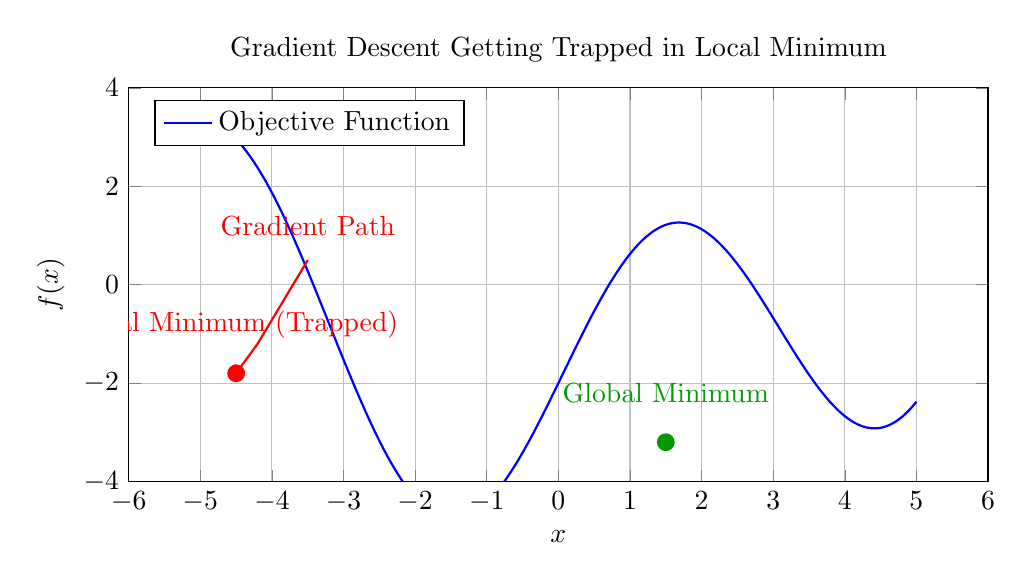
\begin{tikzpicture}
    \begin{axis}[
      width=0.9\textwidth,
      height=5cm,
      scale only axis,
      ymin=-4,
      ymax=4,
      xlabel={$x$},
      ylabel={$f(x)$},
      title={Gradient Descent Getting Trapped in Local Minimum},
      grid=major,
      legend pos=north west,
    ]
    % Multi-modal function
    \addplot[blue, thick, domain=-5:5, samples=200] {sin(deg(x))*3 + 0.1*x^2 - 2};
    \addlegendentry{Objective Function}

    % Local minimum point
    \addplot[red, mark=*, mark size=3pt] coordinates {(-4.5, -1.8)};
    \node[red] at (axis cs:-4.5,-0.8) {Local Minimum (Trapped)};

    % Global minimum point
    \addplot[green!60!black, mark=*, mark size=3pt] coordinates {(1.5, -3.2)};
    \node[green!60!black] at (axis cs:1.5,-2.2) {Global Minimum};

    % Gradient descent path
    \addplot[red, thick, ->] coordinates {(-3.5, 0.5) (-4.2, -1.2) (-4.5, -1.8)};
    \node[red] at (axis cs:-3.5,1.2) {Gradient Path};
    \end{axis}
    \end{tikzpicture}
    \caption{Traditional gradient-based methods follow the local gradient and become trapped in local optima, unable to escape to find the global optimum.}
  \end{figure}

  The second problem with gradient-based methods is that they require the objective function to be differentiable. This becomes a significant limitation when dealing with real-world problems that involve discontinuities, sharp corners, or discrete jumps.
  Such problems are common in engineering design, scheduling, and combinatorial optimization.

  \begin{figure}[H]
  \centering
  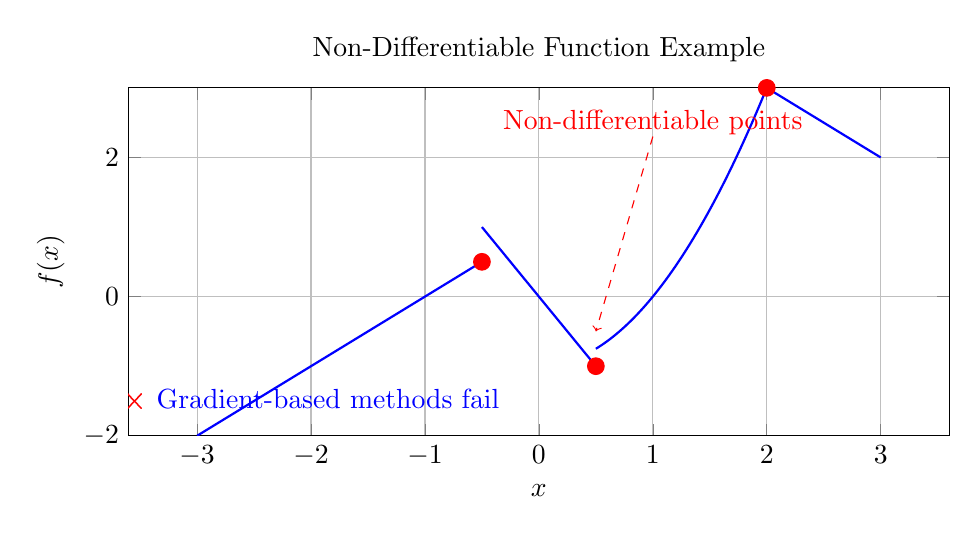
\begin{tikzpicture}
  \begin{axis}[
      width=12cm,
      height=6cm,
      xlabel={$x$},
      ylabel={$f(x)$},
      title={Non-Differentiable Function Example},
      grid=major,
      ymin=-2,
      ymax=3,
  ]
  % Piecewise function with discontinuities
  \addplot[blue, thick, domain=-3:-0.5, samples=50] {x + 1};
  \addplot[blue, thick, domain=-0.5:0.5, samples=50] {-2*x};
  \addplot[blue, thick, domain=0.5:2, samples=50] {x^2 - 1};
  \addplot[blue, thick, domain=2:3, samples=50] {-x + 5};

  % Mark discontinuities
  \addplot[red, mark=*, mark size=3pt, only marks] coordinates {(-0.5, 0.5) (0.5, -1) (2, 3)};
  \node[red] at (axis cs:1, 2.5) {Non-differentiable points};
  \draw[red, dashed, ->] (axis cs:1, 2.3) -- (axis cs:0.5, -0.5);

  \node[blue] at (axis cs:-2, -1.5) {\textcolor{red}{\textbf{×}} Gradient-based methods fail};
  \end{axis}
  \end{tikzpicture}
  \caption{Functions with discontinuities, sharp corners, or discrete jumps cannot be optimized using gradient-based methods.}
  \end{figure}

  % \textbf{How GAs Address This:}
  % \begin{itemize}[leftmargin=*]
  %     \item \textbf{Derivative-free}: GAs only require the ability to evaluate the fitness function, not compute derivatives
  %     \item \textbf{Black-box optimization}: Can handle any function that can be evaluated, regardless of mathematical properties
  %     \item \textbf{Handles discontinuities}: Works equally well with continuous, discrete, or mixed-variable problems
  % \end{itemize}


    While discrete methods such as dynamic programming can handle discontinuities and combinatorial structure, both gradient-based and exact discrete algorithms suffer from the curse of dimensionality: computation typically becomes intractable as problem dimensionality grows.

  \begin{figure}[H]
  \centering
  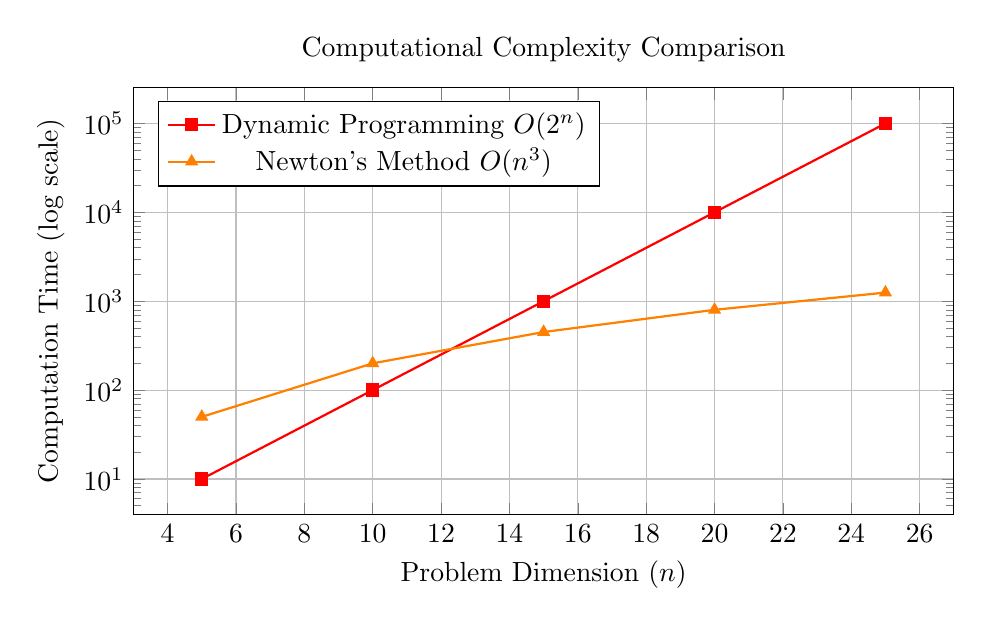
\begin{tikzpicture}
  \begin{axis}[
      width=12cm,
      height=7cm,
      xlabel={Problem Dimension ($n$)},
      ylabel={Computation Time (log scale)},
      title={Computational Complexity Comparison},
      ymode=log,
      legend pos=north west,
      grid=major,
  ]
  % Exponential growth for traditional methods
  \addplot[red, thick, mark=square*] coordinates {
      (5, 10)
      (10, 100)
      (15, 1000)
      (20, 10000)
      (25, 100000)
  };
  \addlegendentry{Dynamic Programming $O(2^n)$}

  % Polynomial growth for Newton
  \addplot[orange, thick, mark=triangle*] coordinates {
      (5, 50)
      (10, 200)
      (15, 450)
      (20, 800)
      (25, 1250)
  };
  \addlegendentry{Newton's Method $O(n^3)$}

  % % Linear-like growth for GA
  % \addplot[green!60!black, thick, mark=*] coordinates {
  %     (5, 20)
  %     (10, 35)
  %     (15, 50)
  %     (20, 65)
  %     (25, 80)
  %     (50, 155)
  %     (100, 305)
  % };
  % \addlegendentry{Genetic Algorithm (approximate)}

  \end{axis}
  \end{tikzpicture}
    \caption{Traditional optimization methods often exhibit exponential or high polynomial growth in computation time as problem dimensionality increases, making them impractical for large-scale problems.}
  \end{figure}

  % \textbf{How GAs Address This:}
  % \begin{itemize}[leftmargin=*]
  %     \item \textbf{Heuristic approach}: Trade optimality guarantee for computational efficiency
  %     \item \textbf{Parallel evaluation}: Population members can be evaluated in parallel
  %     \item \textbf{Scalability}: Computational cost grows more gracefully with problem size
  % \end{itemize}
  %



    Therefore, we can summarize how genetic algorithms effectively address the fundamental limitations of traditional optimization methods in the following table:
  \begin{figure}[H]
  \centering
  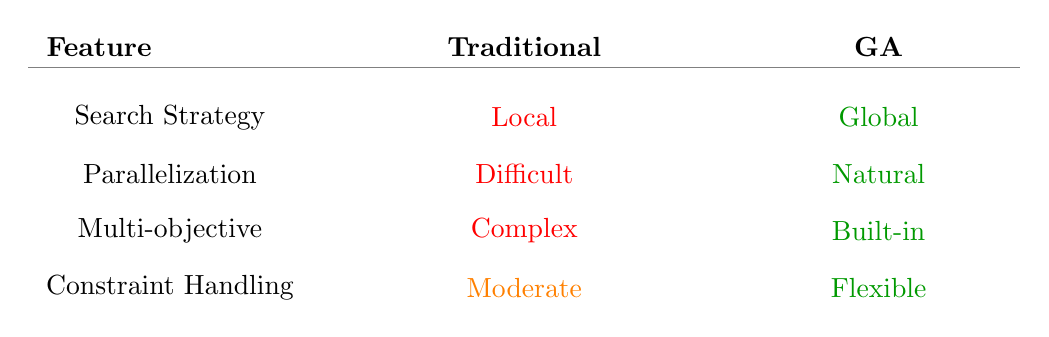
\begin{tikzpicture}[scale=0.9]
      % Comparison rows
      \node[font=\bfseries] at (1, 4) {Feature};
      \node[font=\bfseries] at (7, 4) {Traditional};
      \node[font=\bfseries] at (12, 4) {GA};
      
      \draw[gray] (0, 3.7) -- (14, 3.7);
      
      \node[align=left] at (2, 3) {Search Strategy};
      \node[red] at (7, 3) {Local};
      \node[green!60!black] at (12, 3) {Global};
      
      \node[align=left] at (2, 2.2) {Parallelization};
      \node[red] at (7, 2.2) {Difficult};
      \node[green!60!black] at (12, 2.2) {Natural};
      
      \node[align=left] at (2, 1.4) {Multi-objective};
      \node[red] at (7, 1.4) {Complex};
      \node[green!60!black] at (12, 1.4) {Built-in};
      
      \node[align=left] at (2, 0.6) {Constraint Handling};
      \node[orange] at (7, 0.6) {Moderate};
      \node[green!60!black] at (12, 0.6) {Flexible};
  \end{tikzpicture}
  \caption{Comprehensive comparison showing how GAs address the fundamental limitations of traditional optimization methods.}
  \end{figure}

  \section{Introduction to Evolutionary Computation}
  Evolutionary computation is a family of stochastic, population-based search algorithms inspired by the principles of biological evolution~\cite{holland1975adaptation, eiben2015introduction}. Members of this family operate on a population of candidate solutions and repeatedly apply selection (the principle of survival of the fittest), recombination or crossover (to exchange information between solutions), and mutation (to introduce novel variation). These mechanisms allow evolutionary algorithms to retain and recombine useful solution components while continuously exploring new regions of the search space.

  These properties give evolutionary approaches a number of practical advantages for difficult optimization problems. Because they are derivative-free and only require function evaluations, evolutionary methods are naturally suited to black-box optimization problems, including objective functions that are discontinuous, noisy, non-differentiable, or subject to discrete jumps. Their population-based search confers robustness against local optima and permits straightforward parallel evaluation of candidate solutions, which is valuable for expensive fitness evaluations. While evolutionary algorithms do not generally provide formal optimality guarantees, with appropriate representation and operators they offer reliable heuristic performance across a wide variety of continuous, discrete, and mixed-variable domains.

  The field of evolutionary computation includes several well-established families, each emphasizing different design choices. Genetic Algorithms (GAs) were among the earliest and most influential formulations, emphasizing fixed-length encodings and biologically inspired crossover and mutation operators~\cite{holland1975adaptation, goldberg1989genetic}. Evolution Strategies (ES) concentrate on self-adaptive mutation strategies and are especially effective for real-valued, continuous optimization~\cite{back1996evolutionary}. Evolutionary Programming (EP) historically focused on the evolution of behavioral models and stochastic mutation schemes rather than explicit recombination~\cite{fogel1995evolutionary, fogel2006evolutionary}. Genetic Programming (GP) extends the framework to variable-length structures such as computer programs and expression trees, enabling automatic program synthesis~\cite{koza1992genetic}.

  Evolutionary algorithms have been applied successfully across engineering, science, and business. In engineering design they are used to optimize configurations of complex systems where objective evaluations may be expensive or non-differentiable~\cite{yildiz2023novel}. In machine learning, evolutionary methods have been used both to evolve neural network architectures and to optimize weights when gradient information is unavailable or unreliable~\cite{montana1989training, murad2025hybrid}. Scheduling, timetabling, routing (including the Travelling Salesman Problem), and other combinatorial problems are natural applications because of flexible encodings and bespoke recombination operators that respect problem structure~\cite{gu2022hybrid, fajrin2020multi}. Beyond these domains, evolutionary computation has found roles in bioinformatics, financial modeling, and automated game-play strategy design, demonstrating broad practical utility~\cite{gen2007genetic, sivanandam2008introduction, eiben2015introduction}.

  To make these ideas concrete, consider two compact examples commonly used for pedagogical illustration. A simple toy problem is maximizing the quadratic function $f(x)=x^2$ on the discrete domain $0\leq x\leq31$. With a binary encoding (5-bit chromosomes), repeated cycles of selection, crossover, and mutation concentrate building blocks that represent higher values of $x$ until, typically within a few generations, individuals encoding the optimum ($x=31$) dominate the population. This example highlights how recombination accumulates useful partial solutions (building blocks) even when the initial population is random.

  In a more challenging combinatorial example, the Travelling Salesman Problem (TSP) asks for a shortest tour visiting a set of cities. Genetic Algorithms for TSP use representations and crossover operators that preserve city-order properties (for example, order- or position-based crossovers) and mutation operators that perform local perturbations of tours. While GAs do not guarantee optimality for NP-hard problems like the TSP, they often produce high-quality approximate solutions quickly and can be combined with local search (hybrid approaches) for further improvement.

  \begin{figure}[h]
  \centering
  \includegraphics[width=0.7\textwidth]{figures/buku_ajar_page_4.png}
  \caption{Illustration of GA cycle and variations}
  \label{fig:ga_intro_cycle}
  \end{figure}


    % Note: the detailed, domain-specific examples that previously followed (scheduling, network design, VLSI) were removed here to avoid repetition with the earlier "Applications" section. Key examples remain in the "Applications of Evolutionary Computation" section above.


  Although the Simple Generational Genetic Algorithm serves as the basic framework, various modifications have been developed to improve performance in dealing with problem complexity. Some of these modifications include the following well-studied variants.

  Hybrid Genetic Algorithms combine global evolutionary search with targeted local improvement procedures to exploit the complementary strengths of both paradigms. Typical hybrid designs use a GA for broad exploration while applying deterministic or stochastic local searches (for example, hill-climbing, tabu search, or problem-specific heuristics) to refine selected individuals or the best solutions found so far. By coupling diversification and intensification, hybrid methods often achieve faster convergence and higher-quality results on practical optimization tasks~\cite{majhi2025novel, murad2025hybrid}.

  Adaptive Genetic Algorithms modify control parameters online using feedback from population statistics such as fitness improvement rates, operator success, or measures of genetic diversity. Adaptation can be implemented externally via control rules or internally by encoding parameters within individuals so that evolution itself selects effective settings. These mechanisms reduce manual tuning and help maintain a productive exploration–exploitation balance across different phases of the search~\cite{shams2025resolving, srinivas1994genetic}.

  Parallel Genetic Algorithms exploit modern parallel hardware by distributing computation and/or population structure. Coarse-grained (island) models hold sub-populations on different processors with occasional migration to share information; fine-grained or master–slave models parallelize fitness evaluations to reduce wall-clock time. Parallelism not only accelerates computation but can also enhance search robustness by preserving multiple niches and reducing premature convergence~\cite{eiben2015introduction}.
    \section{Genetic Algorithm Variations}

    Although the simple generational Genetic Algorithm serves as the basic framework, various modifications have been developed to improve performance on complex problems. Common variations include:

    \subsection{Overview}
    \begin{itemize}
        \item \textbf{Hybrid GA:} Combines Genetic Algorithms with local search or other optimization methods to refine promising solutions after global exploration~\cite{majhi2025novel, murad2025hybrid}.
        \item \textbf{Adaptive GA:} Dynamically adjusts parameters such as crossover and mutation probabilities based on population feedback to balance exploration and exploitation~\cite{shams2025resolving, srinivas1994genetic}.
        \item \textbf{Parallel GA:} Splits the population into sub-populations across processors (island models, master-slave, etc.) and periodically exchanges individuals to speed up search and maintain diversity.
    \end{itemize}


  \section{Further Reading}
  \begin{itemize}
      \item Deb, K. (2001). Multi-objective optimization using evolutionary algorithms.
      \item Eiben, A. E., \& Smith, J. E. (2015). Introduction to evolutionary computing.
      \item Goldberg, D. E. (1989). Genetic algorithms in search, optimization, and machine learning.
  \end{itemize}
